%%%%%%%%%%%%%%%%%%%%%%%%%%%%%%%%%%%%%%%%%%%%%%%%%%%%%%%%%%%%%%%%%%%%%%%%%%%%%%%%
\subsection{Ελάττωση σφάλματος μέσω επιλογής σωματιδίων}

Υποθέτοντας ένα κινητό ρομπότ που λειτουργεί στο επίπεδο 2D, τα φίλτρα σωματιδίων διατηρούν
την εκτίμηση της στάσης του ρομπότ σε κάθε χρονικό βήμα
$t$, $\hat{\bm{x}}_t (x, y, \theta)$, εντός ενός χάρτη $M$, με τη μορφή ενός συνόλου από
"σωματιδίων", δηλαδή τυχαίων δειγμάτων από την κατανομή πιθανότητας
$p(\bm{x}_t | \bm{z}_t, M)$, όπου $\bm{z}_t$ είναι ένα διάνυσμα παρατηρήσεων,
που ανιχνεύονται τη χρονική στιγμή $t$ από το ρομπότ μέσω της χρήσης των αισθητήρων του, οι οποίες,
για λόγους απλούστευσης, αποτελείται αποκλειστικά από έναν 2D σαρωτή εμβέλειας. Το
αναπαράσταση της κατανομής $p(\bm{x}_t | \bm{z}_t, M)$ από ένα σύνολο
δειγμάτων οφείλεται στην ουσιαστική δυαδικότητα μεταξύ της πρώτης και της δεύτερης
\cite{bswt}.

Αυτή η ιδιότητα των σωματιδιακών φίλτρων τους επιτρέπει να μπορούν να αναπαραστήσουν πολυτροπικές
κατανομές $-$ μια προϋπόθεση για τον παγκόσμιο εντοπισμό $-$ αλλά, από το
την ίδια λογική, παρέχοντας μια οριστική απάντηση στο ερώτημα του συνδυασμού όλων των
πιθανών υποθέσεων (κάθε σωματίδιο εκφράζει μια διακριτή υπόθεση για την
κατάσταση του ρομπότ εντός $M$) και τον υπολογισμό μιας ενιαίας εκτίμησης της θέσης του ρομπότ.
γίνεται διφορούμενη: στα φίλτρα Kalman, για παράδειγμα, τα οποία είναι αυστηρά μονοτροπικά
εκτιμητές, αντίθετα, η μέση εκτίμηση του φίλτρου για το διάνυσμα της στάσης και η
συνδιακύμανσης αρκούν για τον υπολογισμό της εκτίμησης του $\bm{x}_t$ \cite{kalman},
ενώ στα σωματιδιακά φίλτρα δεν υπάρχει μια ενιαία λύση κλειστής μορφής για αυτή την
πρόβλημα. Η επικρατούσα προσέγγιση για τον υπολογισμό της εκτιμώμενης πόζας και της
διακύμανσης είναι έμμεση και υποθέτει ότι ταυτοποιείται μέσα στην κατανομή των
σωματιδίων τον τρόπο με το μεγαλύτερο συνολικό βάρος, υπολογίζοντας το κέντρο του
και στη συνέχεια υπολογίζει τη διακύμανση γύρω από αυτό. Στην περίπτωση όπου η
εκτίμηση έχει συγκλίνει και η κατανομή έχει γίνει μονοτροπική, αυτή η προσέγγιση
είναι ισοδύναμη με τη μέση τιμή των εκτιμήσεων όλων των σωματιδίων σύμφωνα με τις
ατομικό βάρος.

Η βιβλιογραφία σχετικά με την εξαγωγή ή την εικασία της τελικής στάσης ενός σωματιδίου
φίλτρου με βάση κάποια συγκεκριμένα χαρακτηριστικά σωματιδίων είναι μάλλον ισχνή:
\cite{selection_1} και \cite{selection_2} επικεντρώνονται σε ανθρωποειδή ρομπότ στο
Πρώτον, τη χρονική στιγμή $t$ προσδιορίζουν το σωματίδιο μέσα σε
συγκεκριμένα όρια μεταφορικής και περιστροφικής απόστασης από την εκτίμηση του
πόζα τη χρονική στιγμή $t-1$ με το μεγαλύτερο βάρος. Οι συγγραφείς εκτελούν την επιλογή σε
με αυτόν τον τρόπο προκειμένου να αμβλυνθεί η ασυνέχεια της πόζας. Στη συνέχεια, εάν το βάρος του
της συστάδας των αναγνωρισμένων σωματιδίων δεν είναι μικρό, η τελική πόζα είναι
υπολογίζεται ως το κεντροειδές όλων των σωματιδίων εντός μιας προκαθορισμένης ακτίνας αυτής της
σωματιδίου- ωστόσο, εάν είναι ``μικρό``, μόνο το σωματίδιο με το μεγαλύτερο βάρος
αναφέρεται. Στη συνέχεια θα αποδείξουμε ότι αυτή η τελευταία απόφαση, ενώ
διαισθητική, στην πραγματικότητα δεν είναι σοφή και, επομένως, δεν αποτελεί βιώσιμη υποψηφιότητα για
επέκταση σε άλλες συνθήκες και καταστάσεις εκτός από το πλαίσιο αυτών των
δύο έργων.


Στα φίλτρα σωματιδίων, κάθε σωματίδιο συνδέεται με έναν παράγοντα σπουδαιότητας,
ή βάρος. Το βάρος $w_t^i$ ενός σωματιδίου $i$ τη χρονική στιγμή $t$ ποσοτικοποιεί
την πιθανότητα ενός ρομπότ να έχει παρατηρήσει τις πραγματικές μετρήσεις $\bm{z}_t$
από την εκτιμώμενη θέση του σωματιδίου $\hat{\bm{x}}_t^i(x_i, y_i, \theta_i)$.
Αυτό σημαίνει ότι, δεδομένου ενός χάρτη $M$ πιστότητας στη λειτουργική κατάσταση του ρομπότ
περιβάλλον, όσο πιο ακριβής είναι η εκτίμηση της στάσης του ρομπότ, τόσο πιο
πιο κοντά στην πραγματική θέση του ρομπότ είναι το $\hat{\bm{x}}_t^i(x_i, y_i, \theta_i)$.
$\bm{x}_t(x,y,\theta)$, και επομένως τόσο μεγαλύτερη είναι η πιθανότητα να είναι η
πραγματικές μετρήσεις $\bm{z}_t$ και οι προβλεπόμενες μετρήσεις
$\hat{\bm{z}}_t^i$ συμφωνούν μεταξύ τους είναι. Επομένως, θεωρητικά, μια άμεση
δυσαναλογία υπάρχει μεταξύ του σφάλματος εκτίμησης (η απόκλιση των
εκτιμώμενης στάσης από την πραγματική της τιμή) ενός σωματιδίου και της τιμής του βάρους του:
Όσο μικρότερο είναι το σφάλμα εκτίμησης της πόζας του, τόσο μεγαλύτερο είναι το βάρος του, και αντίστροφα.

Αυτό το τελικό συμπέρασμα, σε αντιπαράθεση με την κυρίαρχη προσέγγιση που συμπεραίνει την
εκτίμησης του φίλτρου, αποτέλεσε το κίνητρό μας για τη διερεύνηση της εξαγωγής πόζας
άλλων μεθόδων από την επικρατούσα. Θεωρητικά, λοιπόν, θα περιμέναμε ότι
η επιλογή σωματιδίων με υψηλό βάρος (που ισοδυναμεί με απόρριψη σωματιδίων με χαμηλό βάρος
σωματιδίων $-$ σωματιδίων των οποίων η εκτίμηση της πόζας εξηγεί τις μετρήσεις $\bm{z}_t$
με πιο μη ικανοποιητικό τρόπο σε σύγκριση με άλλα σωματίδια του πληθυσμού)
για τον υπολογισμό της σύνθετης εκτίμησης του φίλτρου, θα είχε ως αποτέλεσμα
καλύτερες εκτιμήσεις πόζας, δηλαδή εκτιμήσεις πόζας πιο κοντά στην πραγματική τιμή του
θέσης του ρομπότ σε κάθε χρονικό βήμα.
Δεδομένου ότι το βάρος ενός σωματιδίου είναι ένα καθορισμένο, ποσοτικοποιήσιμο και οριστικό μέτρο
της ευθυγράμμισης των εισόδων των αισθητήρων και των αναμενόμενων εισόδων των αισθητήρων υπό την προϋπόθεση της
εκτίμηση της στάσης του σωματιδίου, και η τιμή που αποδίδεται στο βάρος ενός σωματιδίου σε μια
αναλογικό τρόπο, όλες οι μέθοδοι επιλογής που θα καλύψουμε είναι βασισμένες στο βάρος.
μέθοδοι. Περιορίζουμε τις μεθόδους επιλογής μας σε προσεγγίσεις με βάση το βάρος, δεδομένου ότι σε
πλαίσιο των φίλτρων σωματιδίων το βάρος ενός σωματιδίου είναι ο μοναδικός δείκτης
της ποιότητας της εκτίμησής του.

Ας συμβολίσουμε με $\bm{P}_t$ το σύνολο του πληθυσμού των σωματιδίων τη χρονική στιγμή
$t$. Τότε
$\bm{P}_t \equiv \{(\hat{\bm{x}}_t^i, w_t^i)\}, i = 0,1,\dots,|\bm{P}_t|-1$,
όπου $\hat{\bm{x}}_t^i$ είναι η εκτίμηση του $i$-οστού σωματιδίου του ρομπότ
στάσης του ρομπότ τη χρονική στιγμή $t$, και $w_t^i$ είναι το βάρος που σχετίζεται με το σωματίδιο $i$ τη χρονική στιγμή
$t$. Επιπλέον, συμβολίζουμε με
$\overline{W}_t = \dfrac{1}{|\bm{P}_t|}\sum\limits_{i=0}^{|\bm{P}_t|-1} w_t^i$
το μέσο βάρος των σωματιδίων στο $\bm{P}_t$. Στη συνέχεια, διακρίνουμε δύο διακριτά
μεθόδους επιλογής: (α) απόλυτες και (β) σχετικές μεθόδους επιλογής.
Στις μεθόδους απόλυτης επιλογής, ένα απόλυτο ποσοστό ή αριθμός
των σωματιδίων του πληθυσμού $\bm{P}_t$ καλείται να ψηφίσει για τη θέση
εκτίμηση της θέσης τη χρονική στιγμή $t$. Η επικρατούσα μέθοδος υπολογισμού της πόζας είναι μια ειδική περίπτωση
της απόλυτης επιλογής, όπου το ποσοστό των επιλεγμένων σωματιδίων είναι
$100\%$. Στις μεθόδους σχετικής επιλογής, τα σωματίδια επιλέγονται για να
ψηφοφορία υπό την προϋπόθεση της σχέσης των $w_t^i$ και $\overline{W}_t$: για παράδειγμα,
μόνο τα σωματίδια των οποίων $w_t^i > \overline{W}_t$ επιλέγονται να έχουν λόγο στην
συνολική εκτίμηση της στάσης του φίλτρου. Αλγόριθμος \ref{alg:particle_selection}
απεικονίζει τη διαδικασία επιλογής σωματιδίων.

\begin{algorithm}
  \caption{\texttt{particle\_selection}}
  \begin{spacing}{1.2}
  \begin{algorithmic}[1]
    \REQUIRE $\bm{P}_t \equiv \{(\hat{\bm{x}}_t^i, w_t^i)\}$, selection\_manner, fraction
    \ENSURE εκτίμηση της στάσης $\hat{\bm{x}}_t$
    \STATE \textbf{assert} selection\_manner = ABSOLUTE $|\ |$ RELATIVE
    \STATE \textbf{assert} κλάσμα $\in [0,1]$
    \IF {selection\_manner = ABSOLUTE}
      \STATE $\bm{P}_t^\prime \leftarrow $ sort $\bm{P}_t$ by weight $w_t^i$, descending
      \IF {fraction $> 0.0$}
        \STATE $\bm{P}_t^{\prime\prime} \leftarrow \bm{P}_t^\prime[0: \lfloor\text{fraction}\cdot|\bm{P}_t^\prime| \rfloor - 1]$
      \ELSE
        \STATE $\bm{P}_t^{\prime\prime} \leftarrow \bm{P}_t^\prime[0]$
      \ENDIF
    \ENDIF
    \IF {selection\_manner = RELATIVE}
      \STATE $\overline{W}_t \leftarrow \dfrac{1}{|\bm{P}_t|}\sum\limits_{i=0}^{|\bm{P}_t|-1} w_t^i$
      \STATE $\bm{P}_t^{\prime\prime} \leftarrow \hat{\bm{x}}_t^i : w_t^i > \overline{W}_t$
    \ENDIF
    \STATE $\hat{\bm{x}}_t \leftarrow (0,0,0)$
    \FOR {$j = 0 : |\bm{P}_t^{\prime\prime}|-1$}
      \STATE $\hat{\bm{x}_t} \leftarrow \hat{\bm{x}_t} + \bm{P}_t^{\prime\prime}[j].w_t^i \cdot \bm{P}_t^{\prime\prime}[j].\hat{\bm{x}}_t^i$
    \ENDFOR
    \RETURN $\hat{\bm{x}}_t$
  \end{algorithmic}
  \end{spacing}
  \label{alg:particle_selection}
\end{algorithm}

Στον αλγόριθμο \ref{alg:particle_selection}, αν επιλεγεί η απόλυτη επιλογή, η
ο πληθυσμός σωματιδίων ταξινομείται πρώτα με βάση το βάρος (γραμμή 4) σε φθίνουσα σειρά.
Στη συνέχεια, το πρώτο $\lfloor \text{fraction}\cdot|\bm{P}_t^\prime| \rfloor$
σωματίδια επιλέγονται να μεταφερθούν, όπου το κλάσμα $\in [0,1]$
εκφράζει την αναλογία των σωματιδίων που πρέπει να ληφθούν υπόψη (γραμμή 6)- η σύμβαση
κλάσμα $=0$ προορίζεται για την επιλογή του σωματιδίου με το μεγαλύτερο βάρος.
μεταξύ εκείνων του $\bm{P}_t$. Ο συμβολισμός $\bm{P}_t^\prime[a]$ για το σύνολο σωματιδίων
$\bm{\bm{P}_t^\prime}$ δηλώνει το σωματίδιο του $\bm{P}_t^\prime$ στο δείκτη $a$,
ο συμβολισμός $\bm{P}_t^\prime[a$:$b]$ δηλώνει το σύνολο των σωματιδίων που αποτελούνται από
από τα στοιχεία του $\bm{P}_t^\prime$ από τον δείκτη $a$ μέχρι τον δείκτη $b$. Στο
από την άλλη πλευρά, αν επιλεγεί η σχετική επιλογή, το μέσο βάρος του πληθυσμού είναι
υπολογίζεται πρώτα (γραμμή 12), και στη συνέχεια όλα τα σωματίδια των οποίων το βάρος υπερβαίνει αυτό το
περιλαμβάνονται στο σύνολο σωματιδίων που μεταφέρεται προς τα εμπρός (γραμμή 13). Και στις δύο
περιπτώσεις οι υποθέσεις πόζας του συνόλου σωματιδίων που κατέχουν επιλεγμένα σωματίδια,
$\bm{P}_t^{\prime\prime}$, στη συνέχεια υπολογίζεται ο μέσος όρος των βαρών (γραμμή 17) και η προκύπτουσα
πόζα θεωρείται η έξοδος της επιλογής σωματιδίων. Ο συμβολισμός
$\bm{P}_t^{\prime\prime}[j].x$ για σύνολο σωματιδίων $\bm{P}_t^{\prime\prime}$
δηλώνει τη συνιστώσα $x$ του στοιχείου του $\bm{P}_t^{\prime\prime}$ στο δείκτη
$j$.

Ένα δικαιολογημένο ερώτημα/κατηγορία που μπορεί να τεθεί είναι γιατί δεν κρατάμε το σύνολο
μέγεθος του πληθυσμού στο κλάσμα επιλογής και να απαλλαγούμε από την επιλογή
μηχανισμό επιλογής συνολικά. Αυτό θα ήταν δυνητικά καταστροφικό, καθώς η διατήρηση ενός χαμηλότερου
αριθμό σωματιδίων θα αύξανε τον κίνδυνο στέρησης σωματιδίων
\cite{bible}: Καθώς το μέγεθος του πληθυσμού αυξάνεται, αυξάνεται και η πιστότητα του
posterior (\ref{eq:posterior}) με την αληθινή πόζα- αντίστροφα, όσο μικρότερη είναι η
αριθμός των σωματιδίων στο φίλτρο τόσο μεγαλύτερη είναι η πιθανότητα της
απόκλιση. Έτσι, είναι λογικό να προφυλάσσεται από τη στέρηση σωματιδίων με ένα
αυξημένο μέγεθος του πληθυσμού και να χρησιμοποιηθεί ένα καθεστώς επιλογής, ώστε το σύστημα
να αυξάνει την ακρίβειά του χωρίς να θυσιάζει την ποιότητα/ακρίβεια των εκ των υστέρων
ή τη σταθερότητα του MCL.

Αν και θεωρητικά οι παραπάνω μέθοδοι επιλογής είναι ορθές (δεδομένου ότι η επιλογή
βαρύτερα σωματίδια, απορρίπτοντας έτσι τα σωματίδια με κακή εκτίμηση, βελτιώνει την
ποιότητα της συνολικής εκτίμησης), στην πράξη (υποτμήμα
\ref{subsec:disc:particle_selection}) παρατηρούμε ποικίλα ή δυσμενή αποτελέσματα,
τα οποία μπορούν να αποδοθούν (α) στην απώλεια συνολικής πληροφορίας, (β) στην υψηλότερη
βαθμό επιρροής που αποκτούν τα σωματίδια όταν η πληθικότητα του συνόλου ψηφοφορίας είναι
μειώνεται, ή/και (γ) στην απομάκρυνση σωματιδίων με σχεδόν συμμετρικές θέσεις, που υπάρχουν
στον πληθυσμό λόγω της τυχαιότητας που εισάγεται κατά τη διάρκεια του φίλτρου
φάση πρόβλεψης του φίλτρου.

Στην επόμενη ενότητα αιτιολογούμε πώς το χάσμα μεταξύ της εκτιμώμενης στάσης του MCL
και της πραγματικής πόζας μπορεί να μειωθεί περαιτέρω μέσω της αντιστοίχισης σάρωσης.

%%%%%%%%%%%%%%%%%%%%%%%%%%%%%%%%%%%%%%%%%%%%%%%%%%%%%%%%%%%%%%%%%%%%%%%%%%%%%%%%
\subsection{Ελάττωση σφάλματος μέσω ευθυγράμμισης μετρήσεων με σαρώσεις χάρτη}


Στην παρούσα μελέτη επιδιώκουμε να βελτιώσουμε την εκτίμηση ενός φίλτρου σωματιδίων με
διάφορα μέσα: στην προηγούμενη ενότητα σκεφτήκαμε θεωρητικά για το πώς
η επιλογή σωματιδίων με μεγάλη βαρύτητα για τον προσδιορισμό της πόζας εξόδου του φίλτρου
στρέφει το φίλτρο στον υπολογισμό ακριβέστερων εκτιμήσεων. Σε αυτή την ενότητα
θα εξετάσουμε πώς η αντιστοίχιση σάρωσης μπορεί να χρησιμοποιηθεί ως πρόθεση του σωματιδιακού
φίλτρων (ή οποιασδήποτε άλλης τεχνικής εντοπισμού στην πραγματικότητα), έτσι ώστε η τελική εκτίμηση του συστήματος
οι εκτιμήσεις του συστήματος πλησιάζουν περισσότερο στην αλήθεια. Αυτή η τεχνική είναι εμπνευσμένη από
\cite{paid_original} και καλύπτεται λεπτομερέστερα εδώ για τους σκοπούς της
σχολαστικότητας και πληρότητας.

Ας υποθέσουμε ότι ένα ρομπότ εξοπλισμένο με έναν σαρωτή εμβέλειας 2D λειτουργεί σε ένα
καθορισμένο περιβάλλον το οποίο αναπαρίσταται μέσω ενός χάρτη πλέγματος κατάληψης $M$. Ας υποθέσουμε ότι
επίσης ότι τη χρονική στιγμή $t$ το φίλτρο σωματιδίων εξάγει μια εκτιμώμενη θέση
$\hat{\bm{x}}_t(x,y,\theta)$ χρησιμοποιώντας κάποια μέθοδο επιλογής, και ότι μια σάρωση εμβέλειας,
που έχει ληφθεί από την πραγματική θέση του ρομπότ, $L_t^R$, είναι επίσης διαθέσιμη τη χρονική στιγμή
$t$. Τότε, αν κατασκευάσουμε μια εικονική σάρωση $L_t^V$, η οποία είναι η έξοδος μιας
που προέρχεται από τη θέση $\hat{\bm{x}}_t$ που προσομοιώνει την
την αρχή λειτουργίας του πραγματικού σαρωτή \textit{αλλά αυτή τη φορά στο χάρτη
$M$} σε όλο το ίδιο γωνιακό εύρος, είναι δυνατόν με τη σάρωση-αντιστοίχιση των δύο
σαρώσεων εύρους (υποενότητα \ref{subsec:sm_2d}) να προκύψει η μετατόπιση σε ρότα
$\bm{q}_t$ η οποία, αν εφαρμοστεί στην εκτίμηση $\hat{\bm{x}}_t$, θα την κάνει
συμπίπτει με την πραγματική θέση $\bm{x}_t$. Σε αυτό το πλαίσιο, η $L_t^R$ θεωρείται
η σάρωση αναφοράς και $L_t^V$ η σάρωση εισόδου ή δεδομένων.

Ωστόσο, λόγω (α) της παρουσίας θορύβου του αισθητήρα στην $L_t^R$, (β) της
αναπόφευκτης αναντιστοιχίας μεταξύ του περιβάλλοντος λειτουργίας και του χάρτη του $M$, (γ)
της διακριτής φύσης του (υποτίθεται ότι ο $M$ είναι ένας χάρτης πλέγματος πεπερασμένης ανάλυσης),
και (δ) το γεγονός ότι ο χρησιμοποιούμενος σαρωτής-αντισταθμιστής δεν είναι απαραίτητα τέλειος, εμείς
αναμένουμε ότι αυτό που πραγματικά συμβαίνει είναι ότι η εφαρμογή του
$\bm{q}_t$ στην εκτίμηση της στάσης $\hat{\bm{x}}_t$ θα μετακινήσει την εκτίμηση αυτή σε
\textit{a πλησίον} της πραγματικής πόζας και όχι ακριβώς σε αυτήν. Αυτή η εκτίμηση
σφάλμα εξαρτάται από ένα πλήθος παραμέτρων, μεταξύ άλλων, δηλαδή από την ποιότητα της
της οδομετρίας του ρομπότ, την αντιστοιχία του κινηματικού μοντέλου του με την πραγματική δυναμική του,
την ποσότητα του θορύβου των αισθητήρων, την ανάλυση του χάρτη, την ακρίβεια των σαρωτών-ματσογράφων στην
εκτίμησης της μετάθεσης και της περιστροφής, το μέγεθος του πληθυσμού των σωματιδίων, το
η διάταξη του χάρτη σε συνδυασμό με την ικανότητα του σαρωτή-ματ να απορρίπτει τις ακραίες τιμές,
και το μέγιστο εύρος του αισθητήρα σάρωσης.

Ανάλογα με τη διαμόρφωση του MCL, θα θέλαμε να χρησιμοποιήσουμε έναν ανιχνευτή-αντισφαιριστή
που να μπορεί να συμβαδίζει με τη συχνότητα των ενημερώσεων της πόζας, δηλαδή να λειτουργεί
σε πραγματικό χρόνο. Η τεχνική σάρωσης-αντιστοίχισης της επιλογής μας είναι η PL-ICP \cite{plicp}
για τους ακόλουθους λόγους: (α) ξεπερνά την de facto τελευταία λέξη της τεχνολογίας σε
ακρίβεια, τον αριθμό των επαναλήψεων μέχρι τη σύγκλιση και το μέσο χρόνο εκτέλεσης,
και (β) απαιτεί λιγότερες παραμέτρους ρύθμισης, καθώς δεν απαιτεί ούτε σφάλμα
κατώφλια σφάλματος για τη διακοπή της σύγκλισης ούτε μέγιστες εκτιμήσεις της αρχικής εκτίμησης.


%%%%%%%%%%%%%%%%%%%%%%%%%%%%%%%%%%%%%%%%%%%%%%%%%%%%%%%%%%%%%%%%%%%%%%%%%%%%%%%%
\subsection{Ελάττωση σφάλματος μέσω ανάδρασης}


Παρόλο που η εκτίμηση εντοπισμού που εξάγεται από την τεχνική αντιστοίχισης σάρωσης
$\hat{\bm{x}}^{\prime}$ υποφέρει από τις παραπάνω πηγές σφάλματος, είναι,
καταρχήν, ακριβέστερη από εκείνη που εξάγεται από την MCL, $\bm{\hat{x}}$. Αυτό που
σημαίνει ότι το συνολικό σύστημα tandem κατέχει μια εκτίμηση της οποίας η MCL δεν είναι
ενημερωμένη. Συνεπώς, θα ήταν επωφελές να εισαχθεί το $\hat{\bm{x}}^{\prime}$ στο
MCL και, στη βιβλιογραφία, αυτό επιτυγχάνεται με δύο μεθόδους:

\begin{itemize}
  \item Ο πρώτος τρόπος τροφοδότησης του $\hat{\bm{x}}^{\prime}$ στην MCL είναι να
        να την αρχικοποιήσουμε με αυτή την εκτίμηση. Αυτό σημαίνει ότι το σωματίδιο
        πληθυσμός που διατηρείται από το φίλτρο δημιουργείται εκ νέου, με σωματίδια
        να διασκορπίζονται γύρω από το $\hat{\bm{x}}^{\prime}$ με προκαθορισμένη διακύμανση.
        Αυτή είναι η προσέγγιση που ακολουθείται στο \cite{paid_original}, και θα είναι
        θα αναφέρεται στο υπόλοιπο της παρούσας εργασίας ως \textbf{hard loop-closure}.
  \item Ο δεύτερος τρόπος είναι η έγχυση του πληθυσμού των σωματιδίων με ένα σωματίδιο,
        που αντιπροσωπεύει την εκτίμηση $\hat{\bm{x}}^{\prime}$, που χρησιμεύει ως ένα
        διακριτή υπόθεση μεταξύ του τρέχοντος πληθυσμού. Αυτή είναι η προσέγγιση
        που ακολουθείται στην \cite{gangpeng}, και θα αναφέρεται ως \textbf{soft-1
        loop-closure}.
\end{itemize}

Μία από τις ανησυχίες που μπορεί να δημιουργηθούν σχετικά με το σκληρό κλείσιμο βρόχων είναι
ότι δεν είναι ανθεκτικό σε αποτυχίες εντοπισμού: εάν η έξοδος πόζας
από την αντιστοίχιση σάρωσης είναι λανθασμένη, τότε το σύνολο του πληθυσμού του MCL θα είναι
αρχικοποιηθεί γύρω από αυτή τη θέση, με καταστροφικές επιπτώσεις στον εντοπισμό.
Επιπλέον, όσον αφορά το soft-1 loop-closure, η έγχυση ενός
σωματιδίου σε έναν ελάχιστο πληθυσμό αρκετών εκατοντάδων ατόμων χρειάζεται περισσότερους χρόνους για να
από ό,τι αν ένα μεγαλύτερο μέρος του πληθυσμού αντικαθιστούσε το
τη βελτιωμένη εκτίμηση. Συνεπώς, όσο περισσότερα σωματίδια εισάγονται στον πληθυσμό
τόσο πιο επιταχυνόμενη και βελτιωμένη θα είναι η σύγκλισή του (με επιφύλαξη
για την περίπτωση όπου \textit{όλα} τα σωματίδια αντικαθίστανται από πολλαπλά αντίγραφα
της ίδιας εκτίμησης της στάσης- η επισφάλεια αυτής της προσέγγισης έγκειται στην
απουσία της διακύμανσης του φίλτρου).

Παρακινούμενοι από τα παραπάνω γεγονότα, εισάγουμε μια υβριδική στρατηγική κλεισίματος βρόχου, όπου
η εκτίμηση $\hat{\bm{x}}^{\prime}$ εισάγεται στον πληθυσμό των σωματιδίων
ως \textit{μια πληθώρα σωματιδίων}. Η αναλογία τους στο συνολικό τελικό
πληθυσμό είναι σταθερή και έχει οριστεί εκ των προτέρων. Εδώ, υποθέτοντας ότι το μέγιστο
μέγεθος του πληθυσμού είναι $N_{max}$, ότι το επιθυμητό μέγεθος του εγχυόμενου πληθυσμού σε σύγκριση με
με το μέγεθος του πληθυσμού μετά την έγχυσή του είναι $q \in (0,1)$, και ότι τη χρονική στιγμή
$t$ το μέγεθος του πληθυσμού είναι $N_t$, διακρίνουμε τρεις περιπτώσεις:

\begin{itemize}
  \item $N_t = N_{max}$ \\\
        Όταν ο πληθυσμός βρίσκεται στη μέγιστη χωρητικότητά του, τα σωματίδια ταξινομούνται κατά
        κατά φθίνουσα βαρύτητα, και τα χαμηλότερα $\lfloor q N_{max} \rfloor$ σωματίδια
        διαγράφονται, δίνοντας τη θέση τους στην εισαγωγή ίσου αριθμού
        σωματιδίων, όλα κλώνοι του $\hat{\bm{x}}^{\prime}$. Είναι προφανές ότι
        $q N_{max}/N_{max} = q$.
  \item $N_t \leq (1-q) N_{max}$ \\\
        Σε αυτή την περίπτωση, δεν διαγράφονται σωματίδια και $\dfrac{q}{1-q}N_t$
        σωματίδια προστίθενται. Είναι εύκολο να δούμε ότι
        $$\dfrac{\dfrac{q}{1-q}N_t}{\dfrac{q}{1-q}N_t + N_t} = \dfrac{qN_t}{qN_t + (1-q)N_t} = \dfrac{qN_t}{N_t} = q$$
  \item $(1-q) N_{max} < N_t < N_{max}$ \\\
        Στην περίπτωση αυτή, ο πληθυσμός των σωματιδίων $N_t$ ταξινομείται κατά
        κατά φθίνουσα βαρύτητα, το χαμηλότερο $\lfloor N_t - (1-q)N_{max} \rfloor$
        σωματίδια διαγράφονται, και $\lfloor q N_{max} \rfloor$ αντίγραφα των
        της υπόθεσης που εξάγεται από την αντιστοίχιση σάρωσης εισάγονται στο
        πληθυσμό. Και πάλι ο πληθυσμός που εισάγεται είναι, ως ποσοστό,
        $q$ φορές το τελικό μέγεθος του πληθυσμού:
        $$\dfrac{qN_{max}}{N_t - (N_t - (1-q)N_{max}) + qN_{max}} = \dfrac{q N_{max}}{N_{max}} = q$$
\end{itemize}

Η προτεινόμενη στρατηγική ανατροφοδότησης (α) μπορεί να κατευθύνει το σύστημα μακριά από την παγίδα της
ελαττωματικών εκτιμήσεων πόζας που εξάγονται από την αντιστοίχιση σάρωσης $-$ κάτι αναπόφευκτο από το
προσέγγιση του σκληρού κλεισίματος του βρόχου $-$ με τη μη αντικατάσταση του συνόλου των σωματιδίων στο
πληθυσμό του MCL, αλλά αντίθετα διατηρώντας ένα μέρος των καλύτερων εκτιμήσεών του (best in
με την έννοια της υψηλότερης στάθμισης) από τη μία επανάληψη του φίλτρου στην επόμενη, έτσι ώστε,
ακόμη και αν η αντιστοίχιση σάρωσης παράγει μια λανθασμένη εκτίμηση, το φίλτρο μπορεί να ανακτήσει
λόγω της διατήρησης των προηγούμενων εκτιμήσεων που βρίσκονται κοντά στο
πραγματικής στάσης, και (β) επιταχύνει τη σύγκλιση εισάγοντας όχι ένα σωματίδιο $-$ ως
στην περίπτωση της μεθόδου soft-1 loop-closure $-$, αλλά ένα πλήθος από
σωματιδίων καλύτερης εκτίμησης.

Η προτεινόμενη στρατηγική ανατροφοδότησης θα αναφέρεται στο εξής ως
\textbf{soft-}$\bm{p}$ \textbf{loop-closure}, όπου το $p$ εκφράζεται σε ποσοστό
(π.χ. στο καθεστώς του μαλακού κλεισίματος βρόχου $50$, κάθε φορά που η MCL εξάγει ένα
αποτέλεσμα στην PL-ICP, η τελευταία βελτιώνει την εκτίμησή της και εισάγει $-$ και
ενδεχομένως διαγράφει $-$ τόσα σωματίδια όσα απαιτούνται, ώστε η τελική αναλογία
των αντιγράφων της εξόδου του είναι $50\%$ του τελικού συνολικού αποτελέσματος του φίλτρου σωματιδίων
ο όρος soft-1 loop-closure θα διατηρηθεί για την αναφορά στο
αρχική ιδέα της εισαγωγής μόνο ενός σωματιδίου στον πληθυσμό του φίλτρου).

Η δομή του σύνθετου συστήματος απεικονίζεται στο σχήμα
\ref{fig:overall_system}. Η αλγοριθμική μορφή του μηχανισμού ανατροφοδότησης είναι
απεικονίζεται στον αλγόριθμο \ref{alg:feedback_selection} και η διαδικασία του μηχανισμού
εννοιολογικό περιεχόμενο απεικονίζεται σε μορφή μπλοκ στο σχήμα \ref{fig:feedback}.

\begin{figure}[ht]\centering
  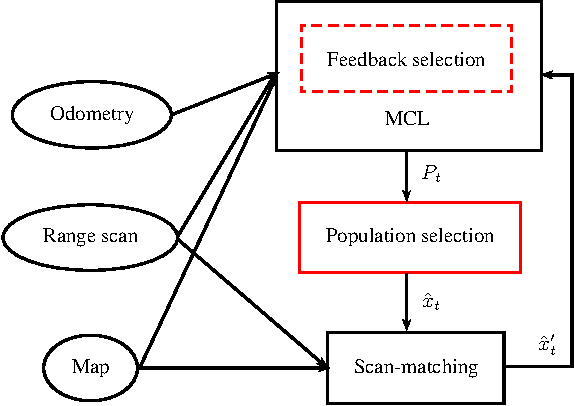
\includegraphics[scale=0.9]{./figures/parts/02/chapters/02/sections/03/overall_system}
  \caption{\small Το συνολικό σύστημα σε δομή μπλοκ. Τα μπλοκ υποδεικνύουν
           υποσυστήματα, ενώ οι ελλείψεις υποδεικνύουν τις εισόδους τους. Το κόκκινο χρώμα είναι
           χρησιμοποιείται για να προσδιορίσει τις συνεισφορές της προσέγγισής μας στο
           στην τελευταία λέξη της τεχνολογίας σε συστήματα tandem με φίλτρα σωματιδίων και
           σάρωσης-αντιστοίχισης.  Εδώ, η αντιστοίχιση σάρωσης αντιμετωπίζεται ως προσθετικό σύστημα του
           MCL. Ο πληθυσμός του MCL $\bm{P}_t$ υπόκειται σε βασισμένο σε βάρος
           επιλογή σε χρόνο $t>0$. Τα επιλεγμένα σωματίδια υπολογίζονται κατά μέσο όρο με βάση το βάρος
           και η προκύπτουσα θέση χρησιμοποιείται ως αρχή μιας εικονικής σάρωσης
           στον χάρτη. Η πραγματική και η εικονική σάρωση αντιστοιχίζονται στη συνέχεια χρησιμοποιώντας
           PL-ICP. Η έξοδος της αντιστοίχισης σάρωσης $\hat{\bm{x}}^{\prime}_t$ είναι, σε
           καταρχήν, πιο ακριβής από εκείνη της MCL, $\hat{\bm{x}}_t$, η οποία
           σημαίνει ότι θα μπορούσε να χρησιμοποιηθεί ως βοήθεια για την MCL
           εντοπισμό του, τροφοδοτώντας τον πίσω σε αυτόν.  Βλέπε κείμενο για τους τρεις τρόπους
           που η ανατροφοδότηση μπορεί να εισαχθεί σε φίλτρα σωματιδίων}
  \label{fig:overall_system}
\end{figure}

\begin{figure}[ht]\centering
  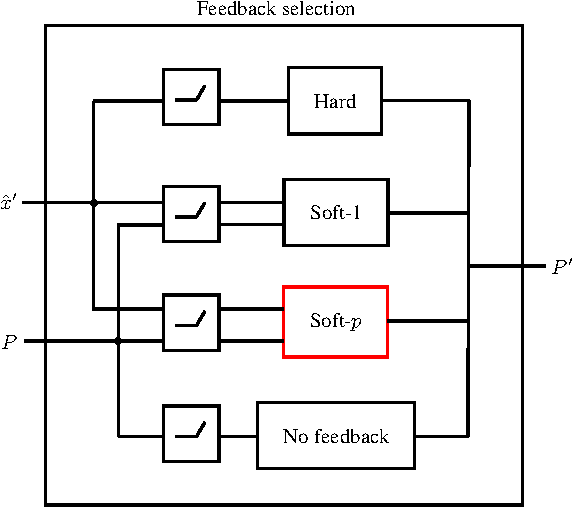
\includegraphics[scale=0.9]{./figures/parts/02/chapters/02/sections/03/feedback}
  \caption{\small Εσωτερικά στην τροποποιημένη έκδοση του MCL, υπάρχουν 4 διαφορετικές
           και αμοιβαία αποκλειόμενοι τρόποι ανατροφοδότησης. Δηλώνεται με
           $\hat{\bm{x}}^{\prime}$ την έξοδο της διαδικασίας σάρωσης-αντιστοίχισης, με
           $\bm{P}$ τον πληθυσμό του φίλτρου κατά τη στιγμή της εκτέλεσης της ανατροφοδότησης,
           και με $\bm{P}^{\prime}$ ο πληθυσμός που εξάγεται από την ανατροφοδότηση: (α) hard
           κλείσιμο βρόχου, όπου ο πληθυσμός του MCL αρχικοποιείται εκ νέου, με
           $\bm{P}^{\prime}$ αποτελούμενο από σωματίδια διασκορπισμένα γύρω από
           $\hat{\bm{x}}^{\prime}$, (β) soft-$1$ κλείσιμο βρόχου, όπου
           $\hat{\bm{x}}^{\prime}$ εισάγεται στο $\bm{P}$ με τη μορφή
           ενός διακριτού σωματιδίου, (γ) μαλακό-$p$ κλείσιμο βρόχου, όπου $p\%$ των
           $\bm{P}^{\prime}$ αποτελείται από κλώνους ενός σωματιδίου
           με πόζα ίση με $\hat{\bm{x}}^{\prime}$ και $(100-p)\%$
           αποτελείται από τα αντίστοιχα σε αριθμό βαρύτερα σωματίδια του
           $\bm{P}$, και (δ) καθόλου ανατροφοδότηση. Το κόκκινο χρώμα χρησιμοποιείται για να
           προσδιορίζει τη συμβολή της προσέγγισής μας σε σχέση με την ανατροφοδότηση.
           στην τελευταία λέξη της τεχνολογίας σε συστήματα φίλτρων σωματιδίων σε συνδυασμό με την αντίστροφη μέτρηση.
           και σάρωσης-αντιστοίχισης. Οι τρόποι ανατροφοδότησης είναι αμετάβλητοι και ορίζονται εκ των προτέρων}
  \label{fig:feedback}
\end{figure}

\begin{algorithm}
  \caption{\texttt{feedback\_selection}}
  \begin{spacing}{1.2}
  \begin{algorithmic}[1]
    \REQUIRE $\bm{P}_t \equiv \{(\hat{\bm{x}}_t^i, w_t^i)\}$, $q$, $\hat{\bm{x}}^\prime_t$, feedback\_manner
    \ENSURE $\bm{P}_{t+1}$
    \STATE \textbf{assert} \\ feedback\_manner $\in \{$HARD, SOFT\_1, SOFT\_P, OPEN $\}$
    \IF {feedback\_manner = HARD}
      \STATE $\bm{P}_{t+1} \leftarrow \overbrace{\{\hat{\bm{x}}^\prime_t\} \cup \{\hat{\bm{x}}^\prime_t\} \cup \dots \{\hat{\bm{x}}^\prime_t\}}^{N_{max}}$
      \STATE Διατάραξη $\bm{P}_{t+1}.\hat{\bm{x}}_t^i$ σύμφωνα με τις αρχικές παραμέτρους MCL
    \ENDIF
    \IF {feedback\_manner = SOFT\_1}
      \IF {$|\bm{P}_t| = N_{max}$}
        \STATE $\bm{P}_t \leftarrow$ Ταξινόμηση $\bm{P}_t$ κατά βάρος, αύξουσα
        \STATE Διαγραφή $\bm{P}_t[0]$
      \ENDIF
      \STATE $\bm{\bm{P}}_{t+1} \leftarrow \bm{P}_t \cup \hat{\bm{x}}^\prime_t$
    \ENDIF
    \IF {feedback\_manner = SOFT\_P}
      \STATE \textbf{assert} $q \in (0,1)$
      \STATE $\bm{S} \leftarrow \{\}$
      \IF {$|\bm{P}_t| \leq (1-q) N_{max}$}
        \STATE $\bm{S} \leftarrow \underbrace{\{\hat{\bm{x}}^\prime_t\} \cup \{\hat{\bm{x}}^\prime_t\} \cup \dots \{\hat{\bm{x}}^\prime_t\}}_{\left\lfloor\dfrac{q}{1-q}|\bm{P}_t|\right\rfloor}$
      \ELSIF {$|\bm{P}_t| = N_{max}$}
        \STATE $\bm{P}_t \leftarrow$ Ταξινόμηση $\bm{P}_t$ κατά βάρος, αύξουσα
        \STATE Διαγραφή $\bm{P}_t[0: \left\lfloor qN_{max} \right\rfloor-1]$
        \STATE $\bm{S} \leftarrow \underbrace{\{\hat{\bm{x}}^\prime_t\} \cup \{\hat{\bm{x}}^\prime_t\} \cup \dots \{\hat{\bm{x}}^\prime_t\}}_{\left\lfloor qN_{max}\right\rfloor}$
      \ELSE
        \STATE $\bm{P}_t \leftarrow$ Ταξινόμηση $\bm{P}_t$ κατά βάρος, αύξουσα
        \STATE Διαγραφή $\bm{P}_t[0: \left\lfloor |\bm{P}_t| - (1-q)N_{max} \right\rfloor-1]$
        \STATE $\bm{S} \leftarrow \underbrace{\{\hat{\bm{x}}^\prime_t\} \cup \{\hat{\bm{x}}^\prime_t\} \cup \dots \{\hat{\bm{x}}^\prime_t\}}_{\left\lfloor qN_{max}\right\rfloor}$
      \ENDIF
      \STATE $\bm{P}_{t+1} \leftarrow \bm{P}_{t} \cup \bm{S}$
    \ENDIF
    \IF {feedback\_manner = OPEN}
      \STATE {$\bm{P}_{t+1} \leftarrow \bm{P}_t$}
    \ENDIF
    \RETURN $\bm{P}_{t+1}$
  \end{algorithmic}
  \end{spacing}
  \label{alg:feedback_selection}
\end{algorithm}

Στον αλγόριθμο \ref{alg:feedback_selection}, εάν ο σκληρά κλειστός βρόχος επιλέγεται ως
η μέθοδος ανατροφοδότησης, το σύνολο των σωματιδίων γεμίζει με $N_{max}$ αντίγραφα
της εξόδου του συστήματος στο προηγούμενο χρονικό βήμα και στη συνέχεια κάθε συνιστώσα κάθε
υπόθεσης θέσης του σωματιδίου υπόκειται σε μικρή διαταραχή σύμφωνα με την
εσωτερικές παραμέτρους του MCL (η ίδια διαδικασία λαμβάνει χώρα κατά την παροχή βανίλιας
MCL με μια εκτίμηση της στάσης του ρομπότ). Εάν έχει επιλεγεί το soft-$1$ κλείσιμο του βρόχου,
η έξοδος του συστήματος εισάγεται στον πληθυσμό ως μία υπόθεση στάσης,
είτε αντικαθιστώντας το σωματίδιο με το χαμηλότερο βάρος όταν ο πληθυσμός βρίσκεται στο
μέγιστο, είτε με απευθείας εισαγωγή διαφορετικά. Εάν επιλέγεται soft-$p$ loop-closure
επιλεγεί, το σύνολο σωματιδίων $\bm{S}$ γεμίζει με τόσα αντίγραφα του συστήματος
εξόδου που απαιτούνται, έτσι ώστε μετά την εισαγωγή η αναλογία τους επί του
σε ολόκληρο τον πληθυσμό είναι $q$ (ή $p = 100 q\%$). Στον ανοικτό βρόχο ο πληθυσμός
δεν υφίσταται καμία τροποποίηση. Οι ενδείξεις ``HARD'', ``SOFT\_1'', ``SOFT\_P'', και
``OPEN" είναι συντομογραφία των τεσσάρων επιτρεπτών τρόπων ανάδρασης, δηλαδή
σκληρό κλείσιμο βρόχου, μαλακό κλείσιμο βρόχου $1$, μαλακό κλείσιμο βρόχου $p$ και όχι
ανατροφοδότηση, αντίστοιχα.

Το εισαγόμενο συνολικό σύστημα είναι πιο ευέλικτο από έναν συνδυασμό tandem των
vanilla MCL με δειγματοληψία KLD και προσαρμογή σάρωσης, καθώς το τελευταίο είναι ένα
ειδική περίπτωση της πρώτης: επιλέγοντας $100\%$ των σωματιδίων από
του πληθυσμού του MCL για την εξαγωγή της εκτίμησης της στάσης του και χωρίς ανατροφοδότηση κάνει
το συνολικό σύστημα εξελίσσεται στην απλούστερη περίπτωση διαμόρφωσης της
εισαγόμενου συστήματος, δηλαδή αυτό που τώρα θεωρείται MCL με δειγματοληψία KLD.
Επιπλέον, και οι δύο προσεγγίσεις που παρουσιάζονται στις \cite{paid_original} και
\cite{gangpeng} αποτελούν ειδικές διαμορφώσεις του προτεινόμενου συστήματος.

Στη συνέχεια, όταν αναφερόμαστε στην πόζα που εξάγεται από το MCL αναφερόμαστε σε
$\hat{\bm{x}}_t$, και όταν αναφερόμαστε στην έξοδο πόζας από το σύστημα, ή στην
σύνθετο σύστημα ή το συνολικό σύστημα, αναφερόμαστε σε $\hat{\bm{x}}^{\prime}_t$.
